\subsection{Notifications Module}
\par{This module will be responsible for the handling of User notifications.}
\subsubsection{Scope}
\par{Users will have the option of subscribing to Forum content and receiving notifications on this specific content via email.}

%\begin{figure}[h!]
%\includegraphics[width=\linewidth]{}
%\caption{Scope of the Buzz-Notification Module.}
%\end{figure}

\subsubsection{Use cases}
\subsubsection*{Add notification}
\par {The user will be able to make additions to the list of content he/she wants notifications on. This will be handled in the form of subscriptions.}
\subsubsection*{Remove notification}
\par{This involves the removal of subscriptions when a user does not want to receive anymore notifications on the said content or posts.}

\subsubsection{Service Contracts}
\par{The notification requests will need to be of a specific type and properly validated before being processed. The request will fail if it does not meet its specified prerequisites. In order for a notification request to be passed on to the server, the user needs to already exist on the database. If this requirement is not met, a notification request will fail. Once a user has subscribed to receive notification on a said topic the following will be accomplished:}
\medskip
\begin{itemize}
\item Notify user of new posts for the subscribed thread.
\item Notify user of new responses made for the subscribed thread.
\item Notify user of new bounty-posts made for the subscribed thread.
\end{itemize}

\subsubsection{Technologies}
\begin{itemize}
\item The linking of the notification with the thread or post it is associated with will be done using JavaScript.This will allow for dynamic posting of notifications, without the administrator having to manually create every notification.
\item Google Email is an API with a capacity to service a number of email within a limit. The API will be ideal to provide messaging capacity for the system without having to implement email servers internally.
\end{itemize}

\subsubsection{Domain Model}
\par{The domain model for the notifications module is represented in figure 6 below:}

\begin{figure}[h!]
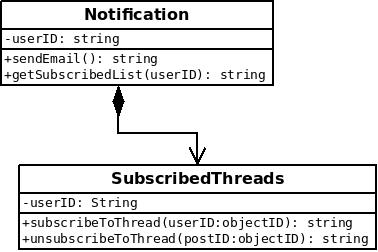
\includegraphics[width=\linewidth]{Diagrams/NotificationDM.jpeg}
\caption{Domain model of Notifications}
\end{figure}

\begin{figure}[h!]
%\includegraphics[width=\linewidth]{}
\caption{Domain model of Notifications}
\end{figure}